\documentclass[12pt]{article}
  \usepackage{geometry}
 \usepackage[round]{natbib}
 \usepackage{graphicx}
 \geometry{a4paper}
  \usepackage[T1]{fontenc}
  \usepackage[utf8]{inputenc}
  \usepackage{authblk}
  \usepackage[running]{lineno}
  \usepackage{setspace}
  \usepackage{booktabs}
  \usepackage{tabularx}
  \usepackage{chngpage}
  \usepackage{amsmath}
  \usepackage{amssymb}
  \usepackage[hidelinks]{hyperref}
 \usepackage[textsize=tiny]{todonotes}


\usepackage{natbib} %package for bibliography

%   \doublespacing
% \raggedright
\title{A Meta-analysis of Longevity Estimates of Mosquito Vectors of Disease: Figures}
\author{Ben Lambert, Ace North, Charles Godfray}

\begin{document}
\maketitle

\begin{figure}[h]
	\centerline{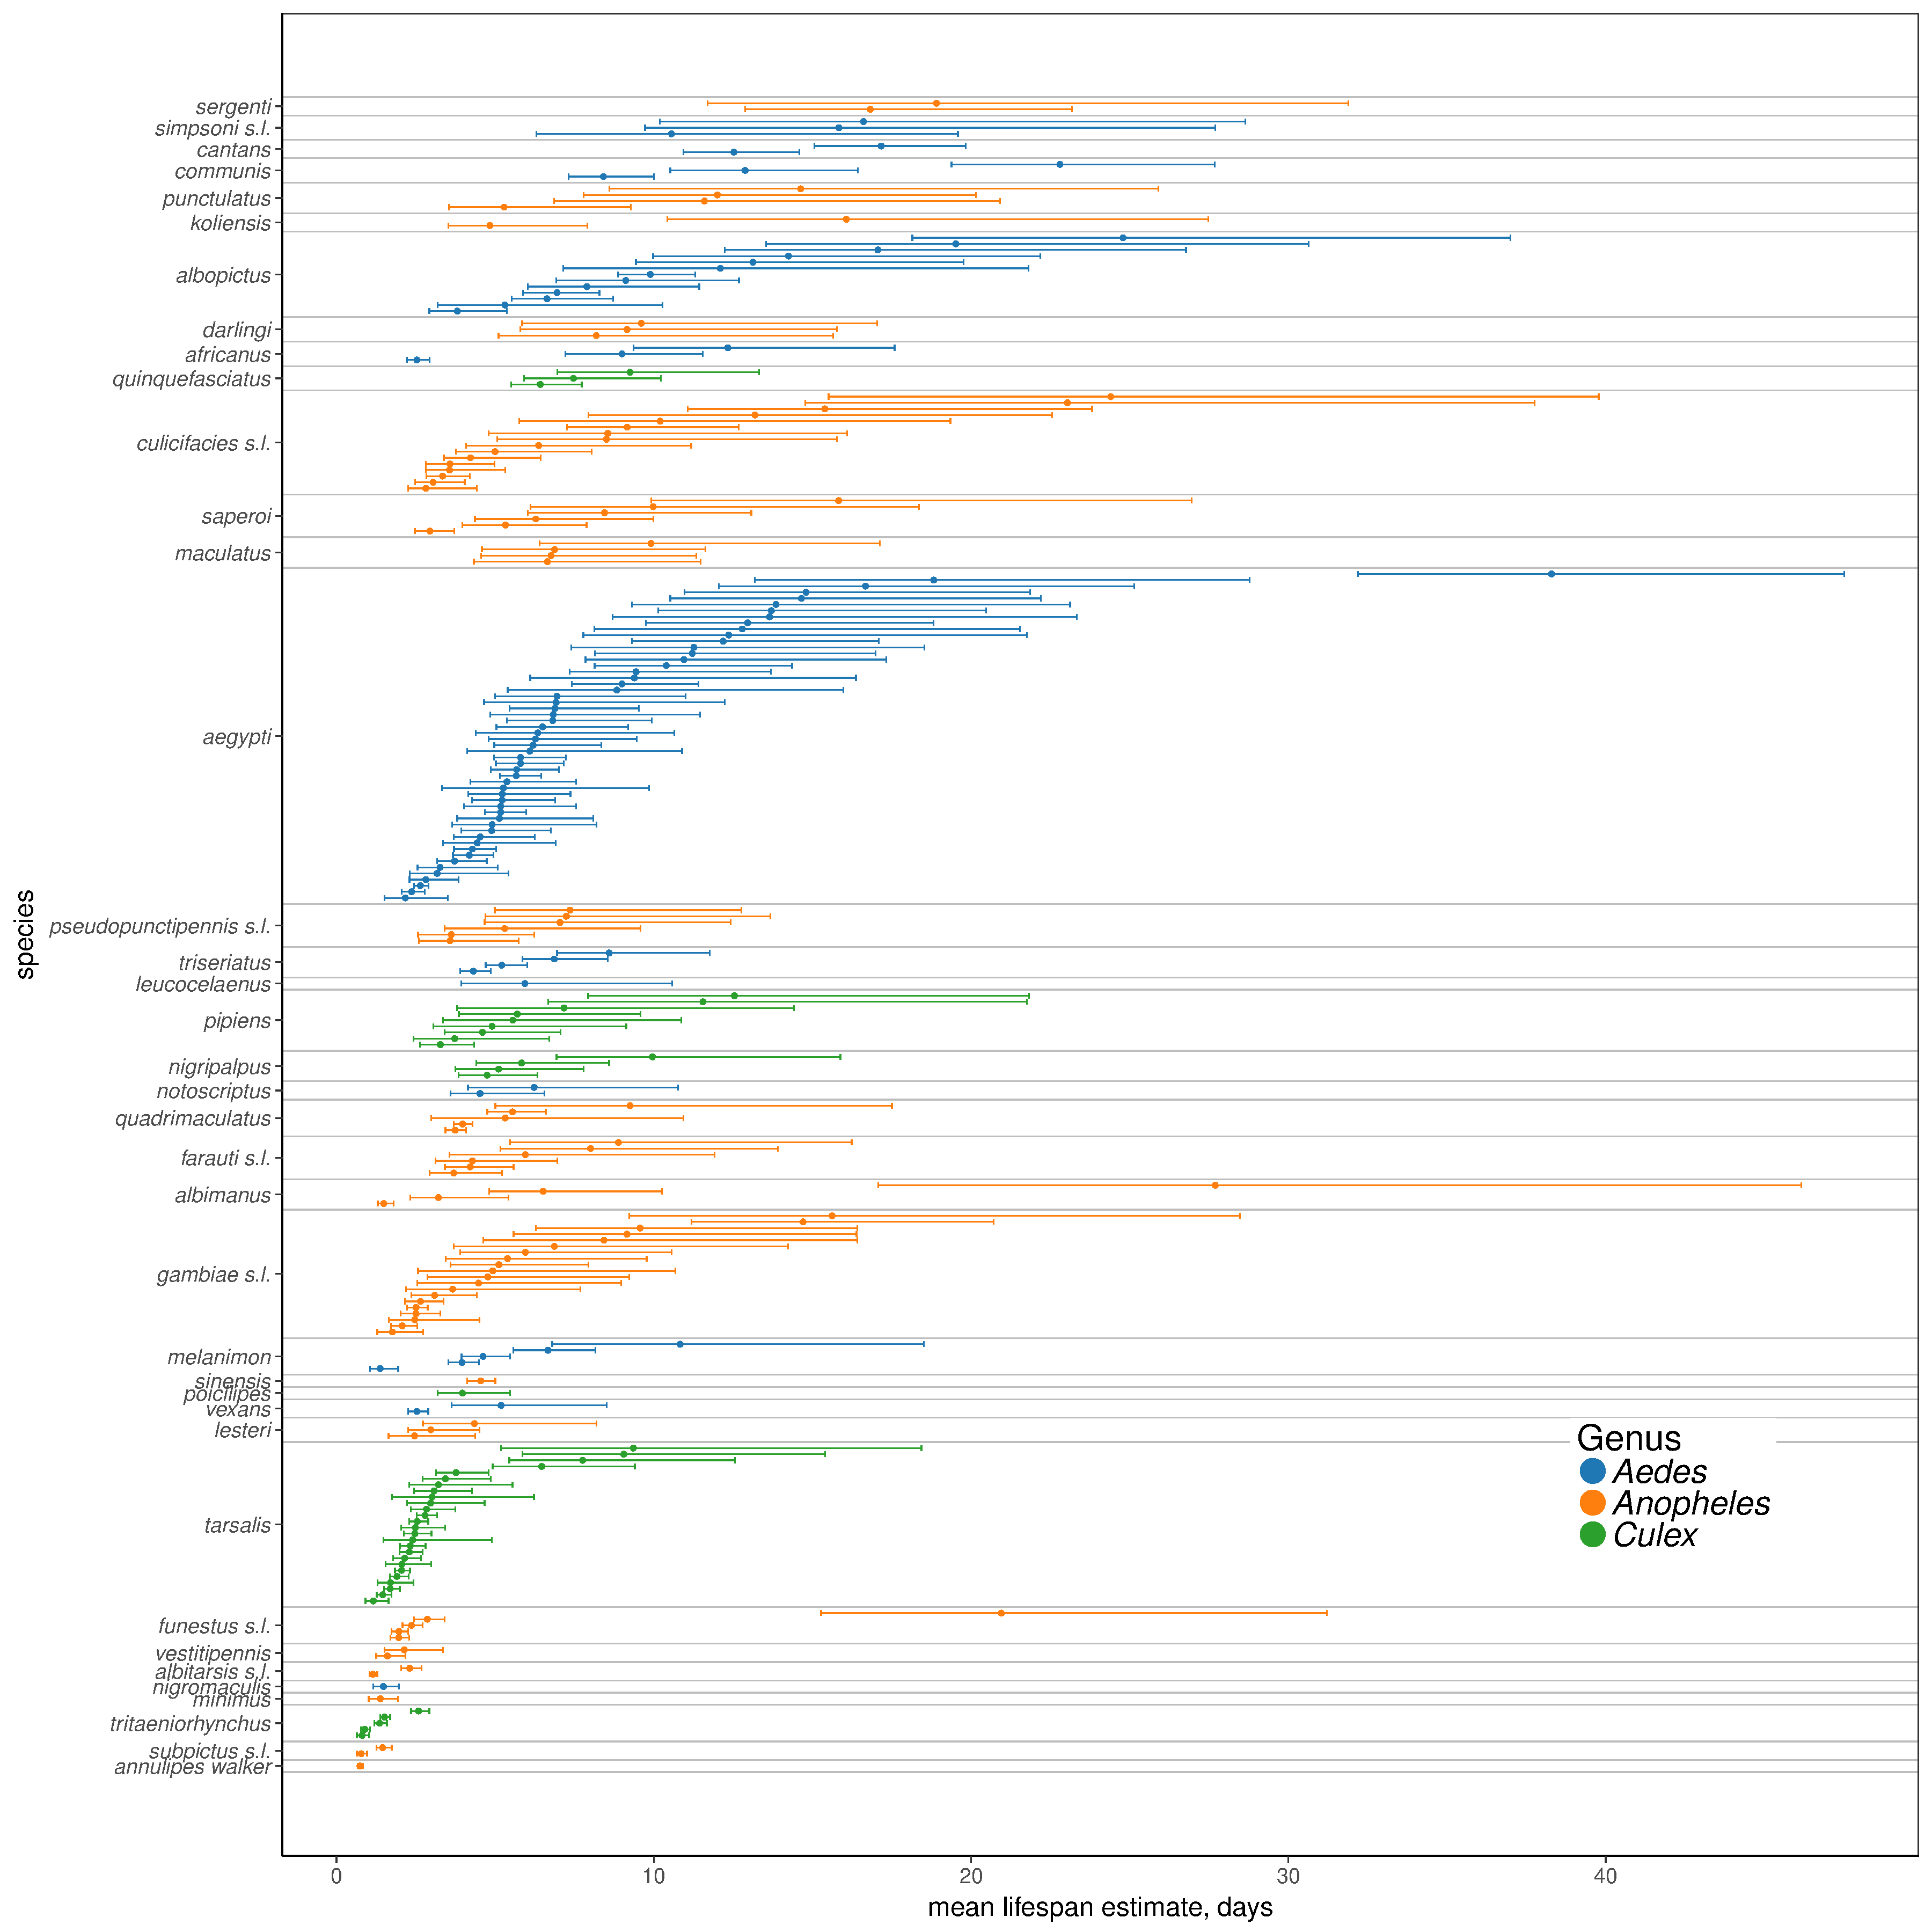
\includegraphics[width=1\textwidth]{./Figure_files/mrr_individualEstimates_allSpecies_withoutBalabacensis.pdf}}
	\caption{\textbf{Individual time-series estimates of adult mosquito mean lifespan from the MRR analysis ordered by species.} The middle point shows the median estimates, and the left and right box whiskers show the 25\%, and 75\% posterior quantiles respectively. All estimates were obtained using the non-hierarchical exponential survival model as described in text.}
	\label{fig:mrr_lifespan_individualEstimates}
\end{figure}

\begin{figure}[h]
	\centerline{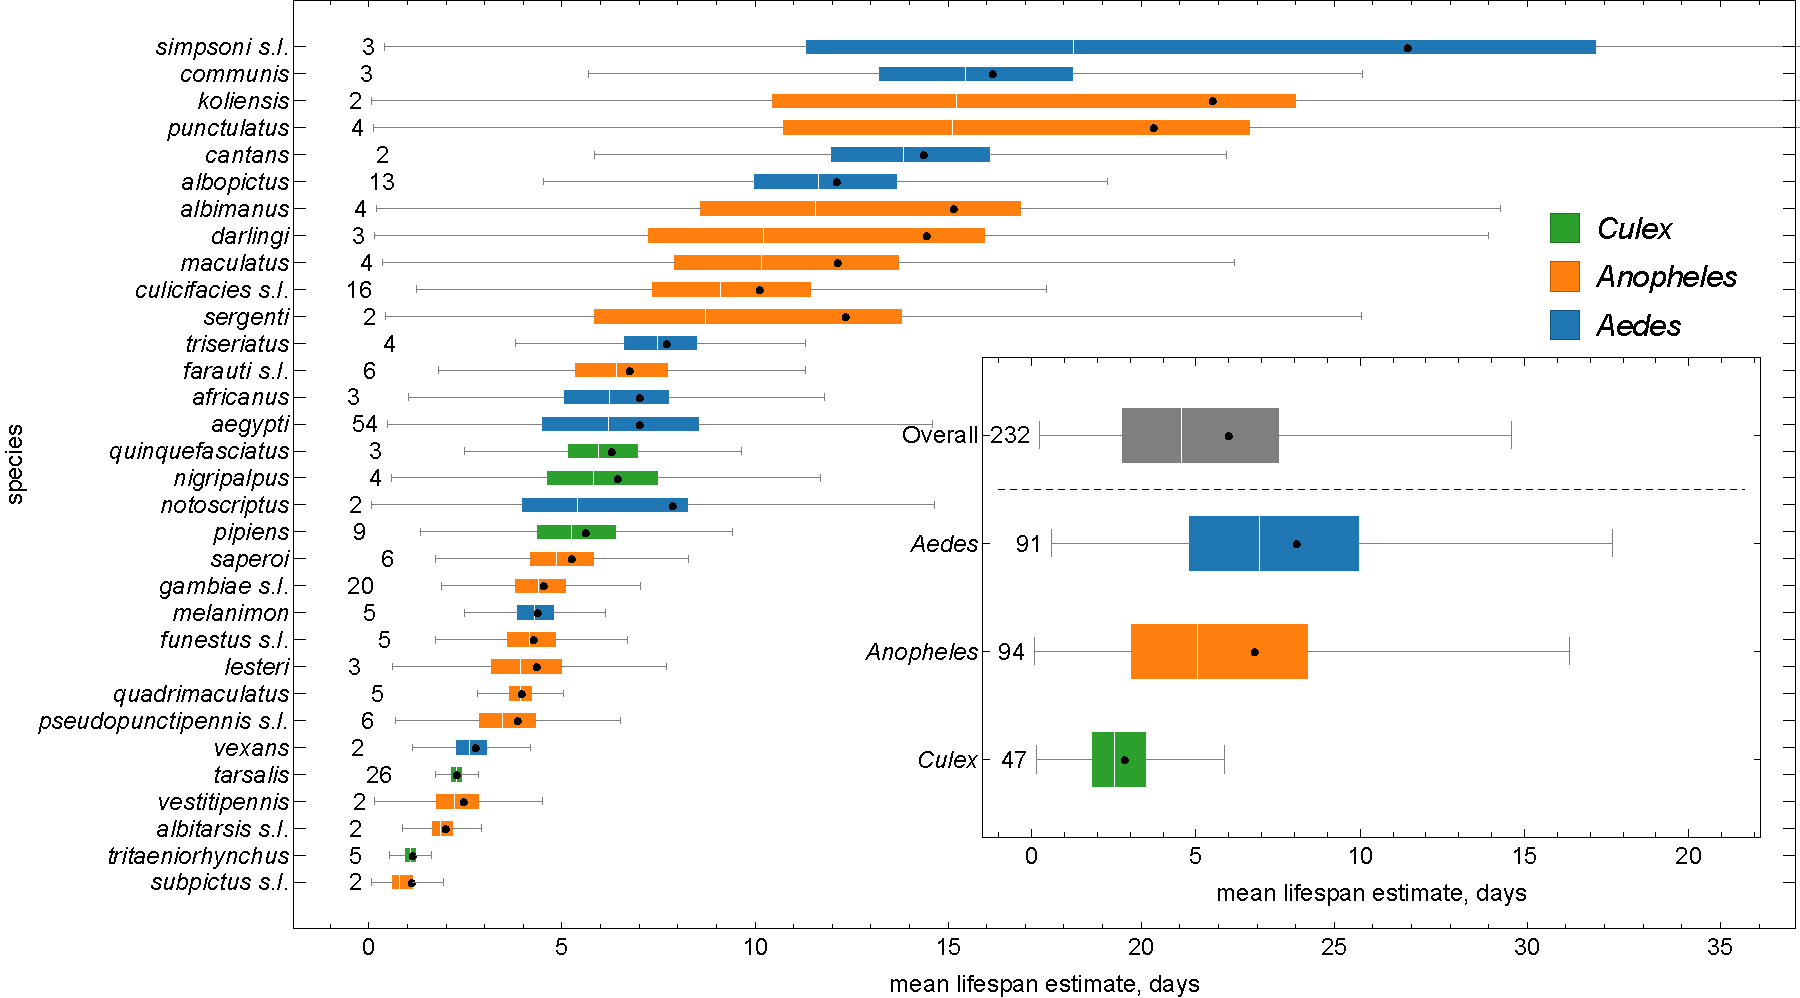
\includegraphics[width=1\textwidth]{./Figure_files/mrr_lifetimes_final_female_without_sugar_not_blood.pdf}}
	\caption{\textbf{Posterior estimates of female mosquito mean lifespan across species, genus and overall groupings as determined from the MRR data.} The lifespans shown are for mosquitoes that were not fed with sugar or blood before release. The middle line in each box shows the median estimates and the solid dot indicates the mean. The left and right box edges show the 25\%, and 75\% posterior quantiles respectively. The whiskers show the range of the data, excluding points lying more than 1.5 times the interquartile range away from each edge of the box. The numbers before the start of the left whisker indicate the number of individual time-series within each species. All estimates were obtained using the hierarchical exponential survival model.}
	\label{fig:mrr_lifespans}
\end{figure}

\begin{figure}[h]
	\centerline{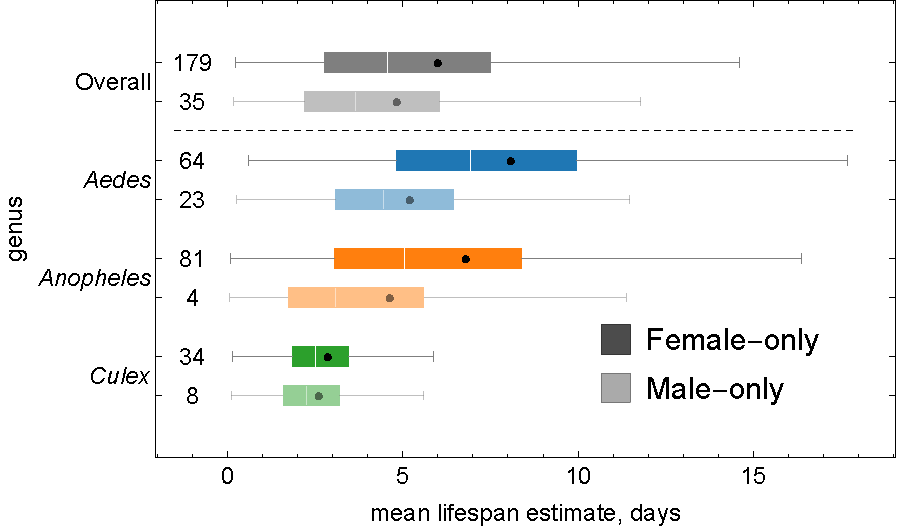
\includegraphics[width=1\textwidth]{./Figure_files/mrr_sexDifferences_without_sugar_nor_blood.pdf}}
	\caption{\textbf{Posterior estimates of female and male mosquito mean lifespan across species, genus and overall groupings as determined from the MRR data.} The lifespans shown are for mosquitoes that were not fed with sugar or blood (for females) before release. The middle line in each box shows the median estimates and the solid dot indicates the mean. The left and right box edges show the 25\%, and 75\% posterior quantiles respectively. The whiskers show the range of the data, excluding points lying more than 1.5 times the interquartile range away from each edge of the box. The numbers before the start of the left whisker indicate the number of individual time-series within each species. All estimates were obtained using the hierarchical exponential survival model.}
	\label{fig:mrr_sexDifferences_without_sugar_nor_blood}
\end{figure}

\begin{figure}[h]
	\centerline{\includegraphics[width=1\textwidth]{./Figure_files/mrr_lifeSpanVsTemperature.pdf}}
	\caption{\textbf{Posterior estimates of mean mosquito lifespan for each time-series versus the average monthly temperature for each study location and date.} The markers show the median posterior estimates, with the lower and upper bounds indicating the 25\% and 75\% quantiles, respectively. The black line shows a regression line with linear and quadratic terms estimated using the median posterior lifetimes, with the grey shading indicating 95\% confidence intervals. All estimates of lifespan were obtained using the non-hierarchical exponential survival model.}\label{fig:mrr_temperature}
\end{figure}

\begin{figure}[h]
	\centerline{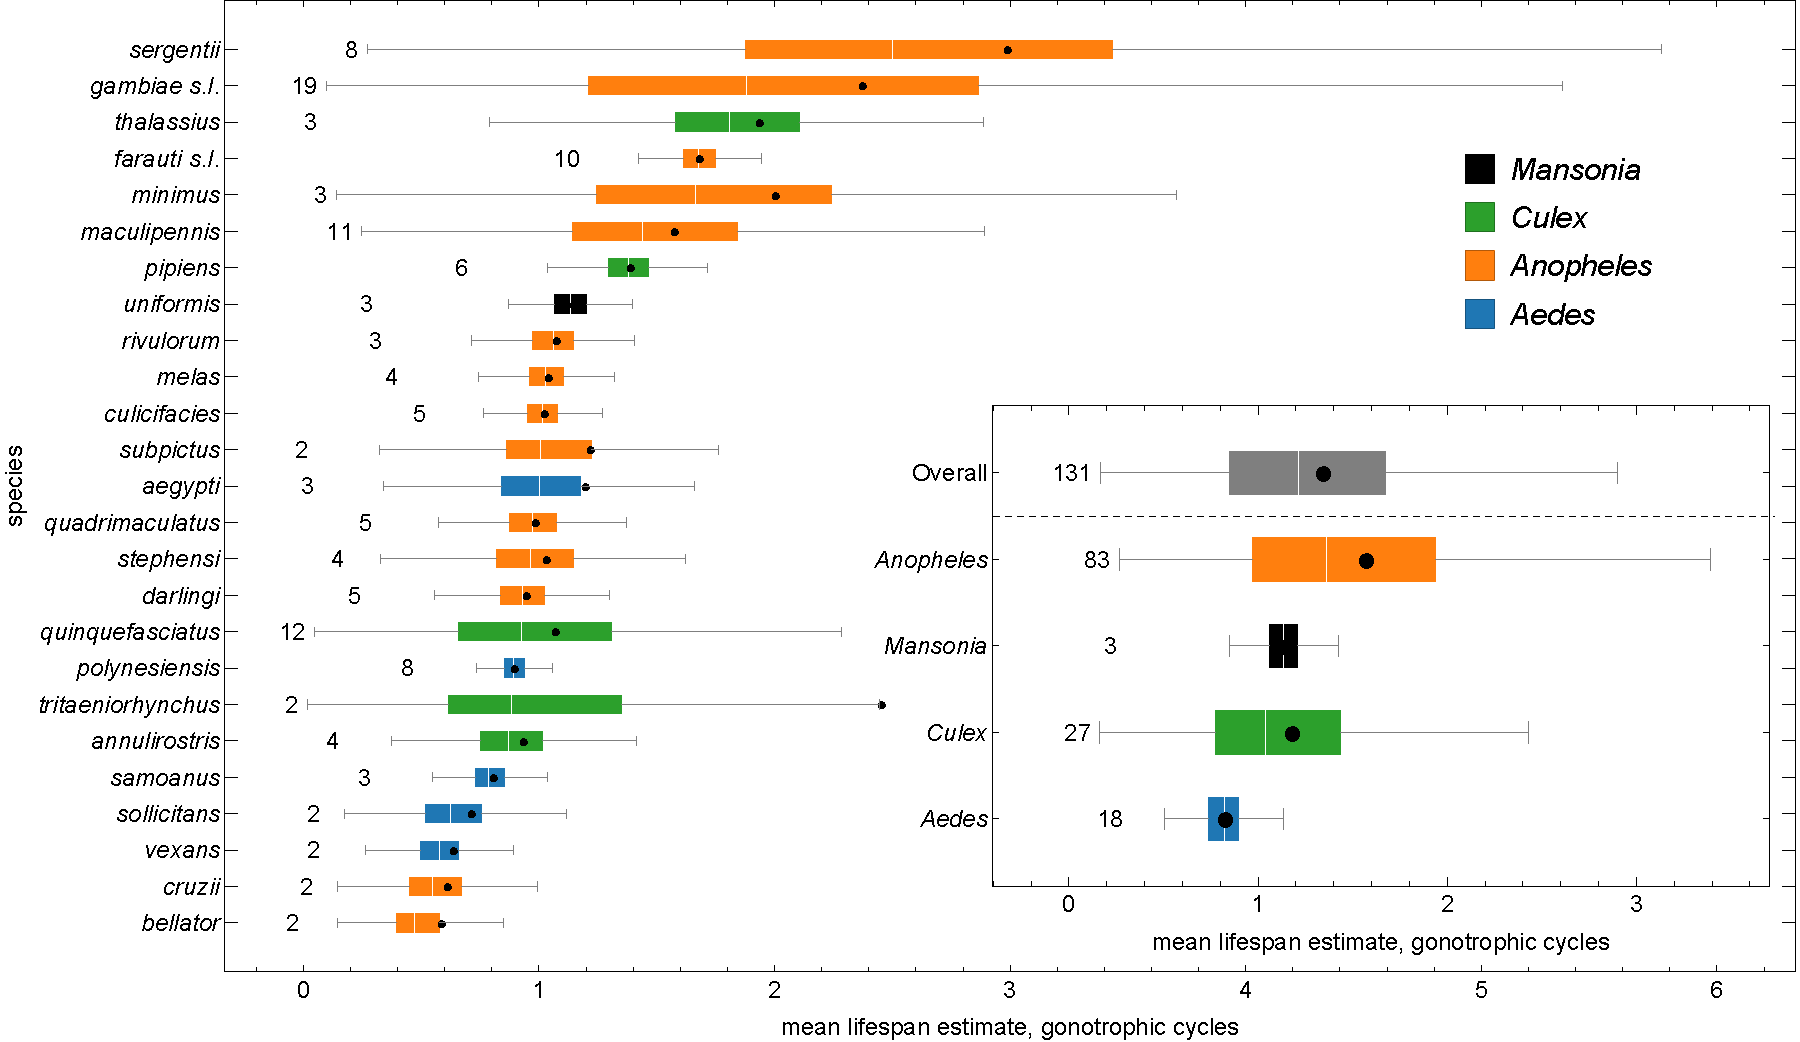
\includegraphics[width=1\textwidth]{./Figure_files/dissection_lifetimes_exponential.pdf}}
	\caption{\textbf{Posterior estimates of female mosquito mean physiological lifespan across species, genus and overall groupings as determined from the dissection data.} The lifespans shown are for mosquitoes that were not fed with sugar or blood (for females) before release. The middle line in each box shows the median estimates and the solid dot indicates the mean. The left and right box edges show the 25\%, and 75\% posterior quantiles respectively. The whiskers show the range of the data, excluding points lying more than 1.5 times the interquartile range away from each edge of the box. The numbers before the start of the left whisker indicate the number of individual time-series within each species. All estimates were obtained using the hierarchical exponential survival model.}
	\label{fig:dissection_lifetimes_exponential}
\end{figure}

\begin{figure}[h]
	\centerline{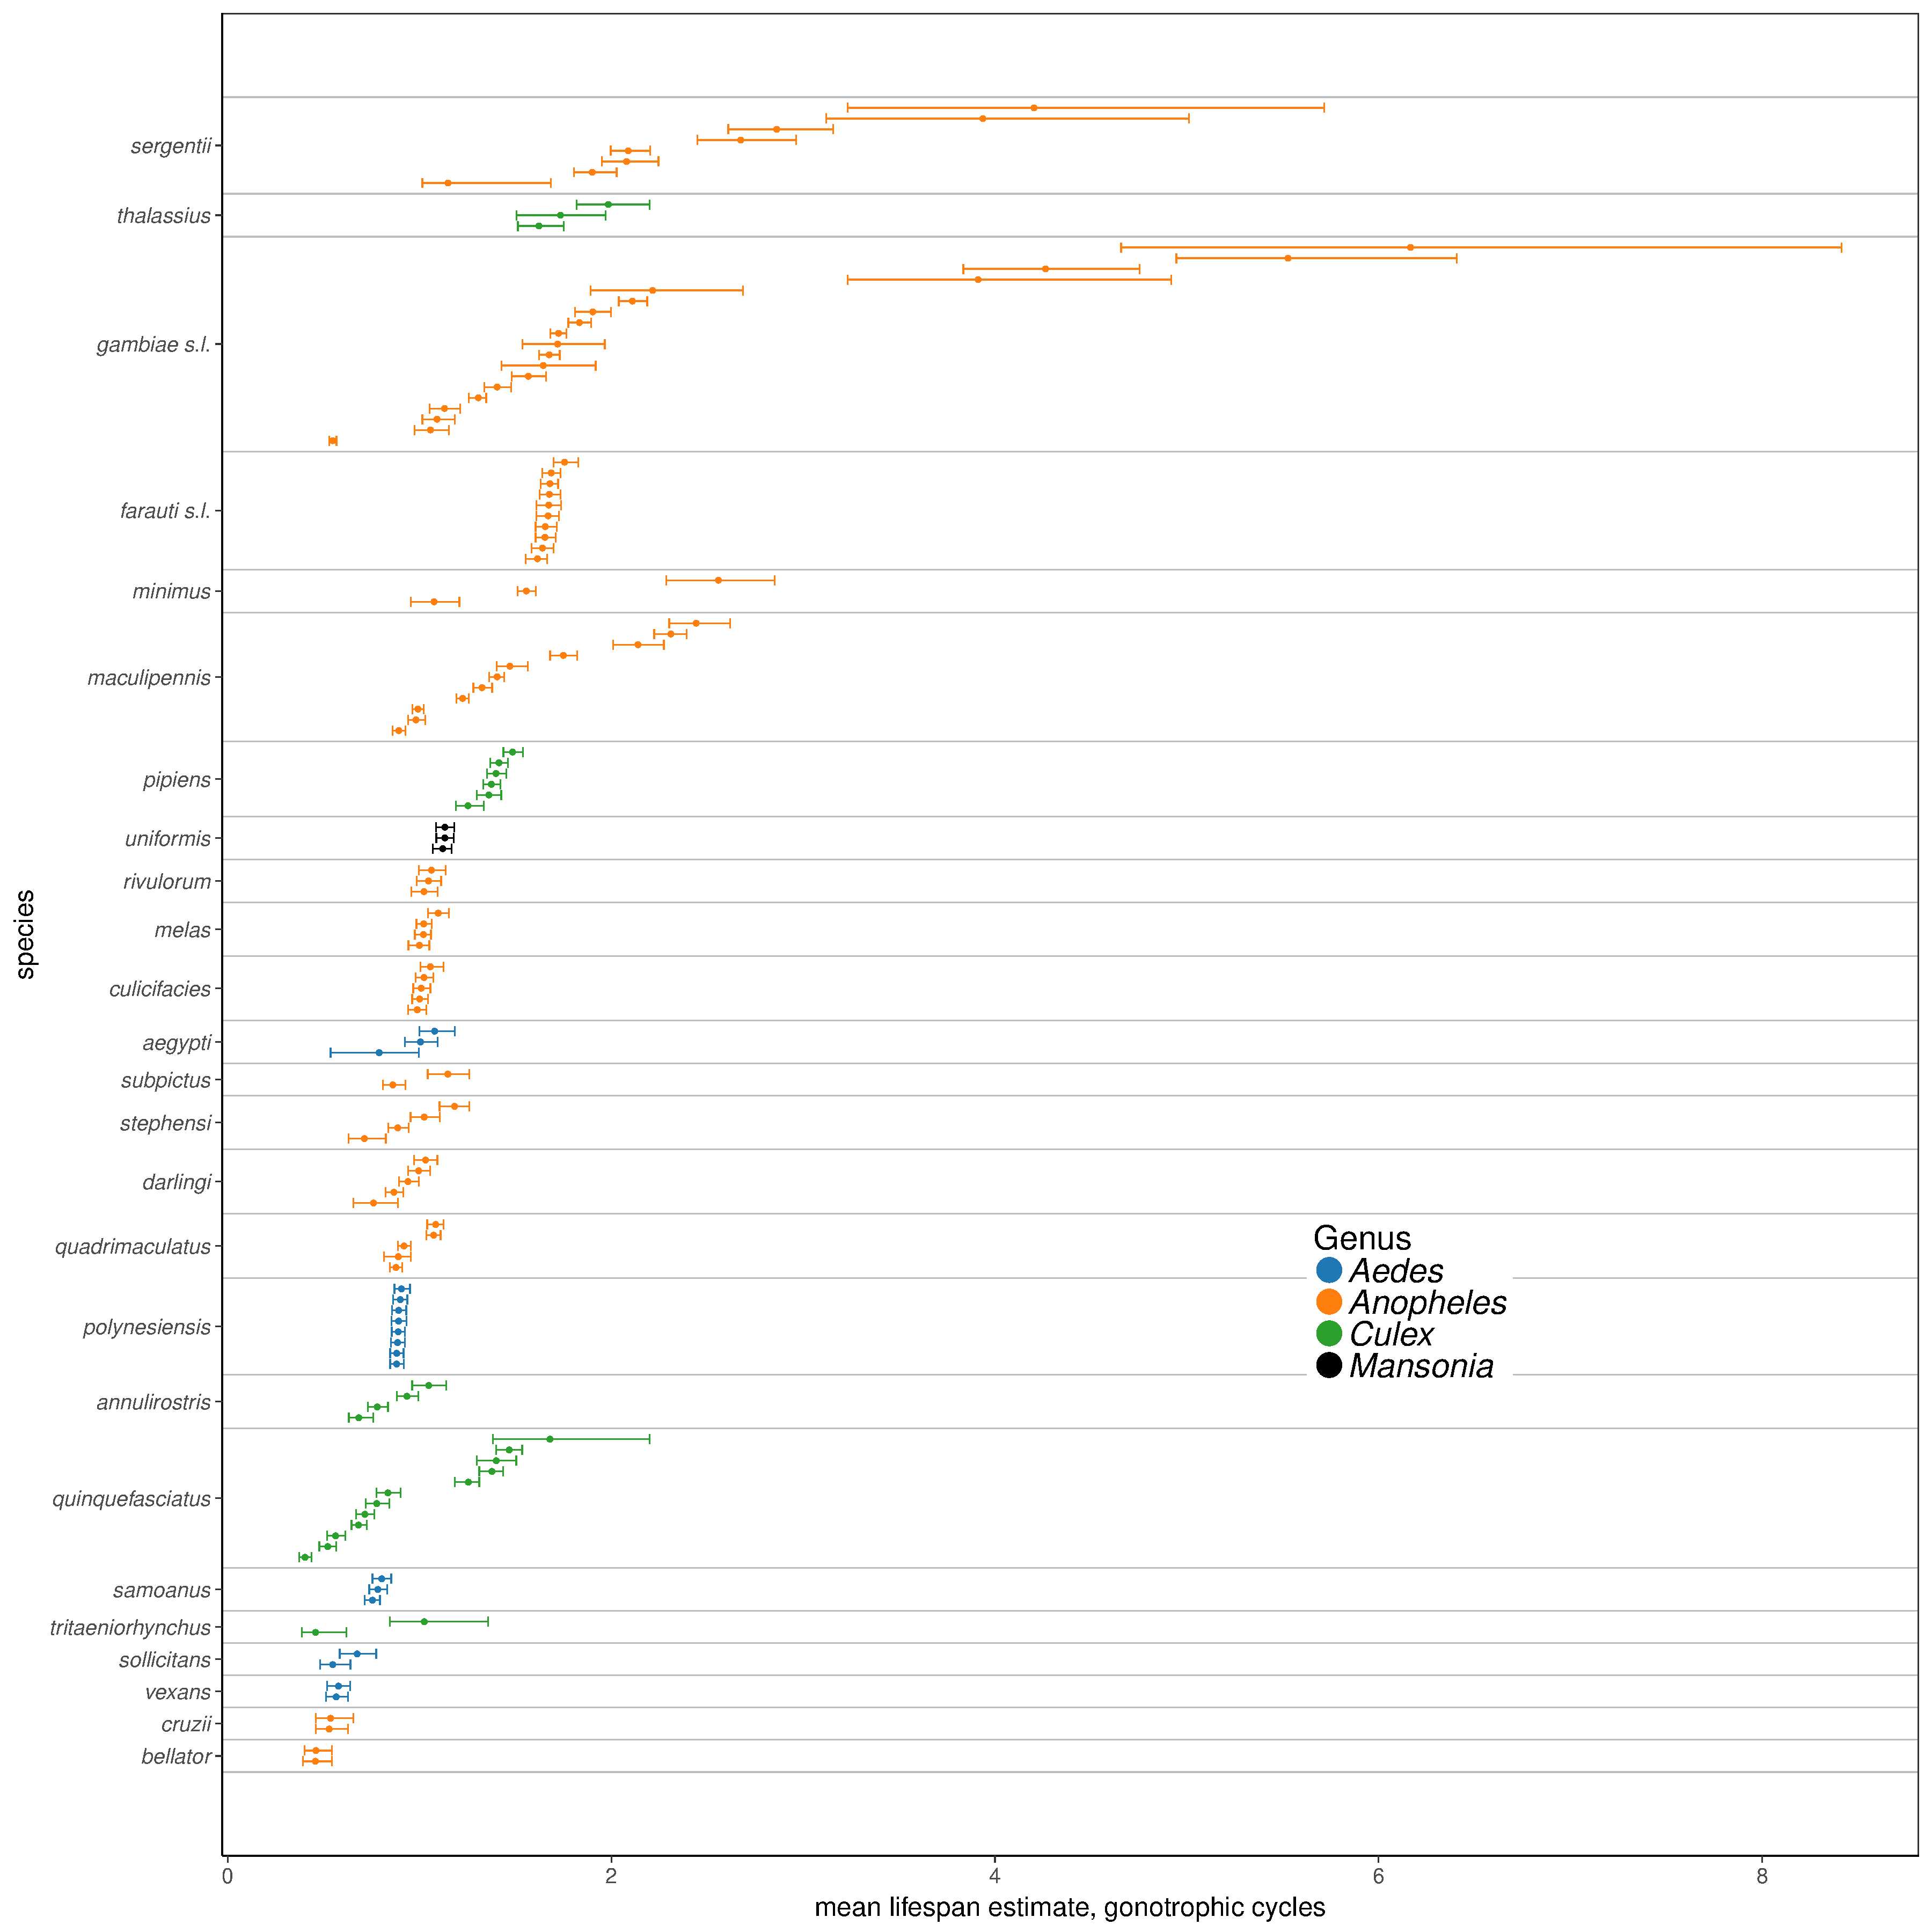
\includegraphics[width=1.3\textwidth]{./Figure_files/dissection_individualEstimates_allSpecies.pdf}}
	\caption{\textbf{Individual time-series estimates of adult mosquito mean lifespan ordered by species median as determined from the dissection data.} The middle line in each box shows the median estimates. The left and right box whiskers show the 25\%, and 75\% posterior quantiles respectively. All estimates were obtained using the non-hierarchical exponential survival model.}
	\label{fig:dissection_individualEstimates_allSpecies}
\end{figure}

\begin{figure}[h]
	\centerline{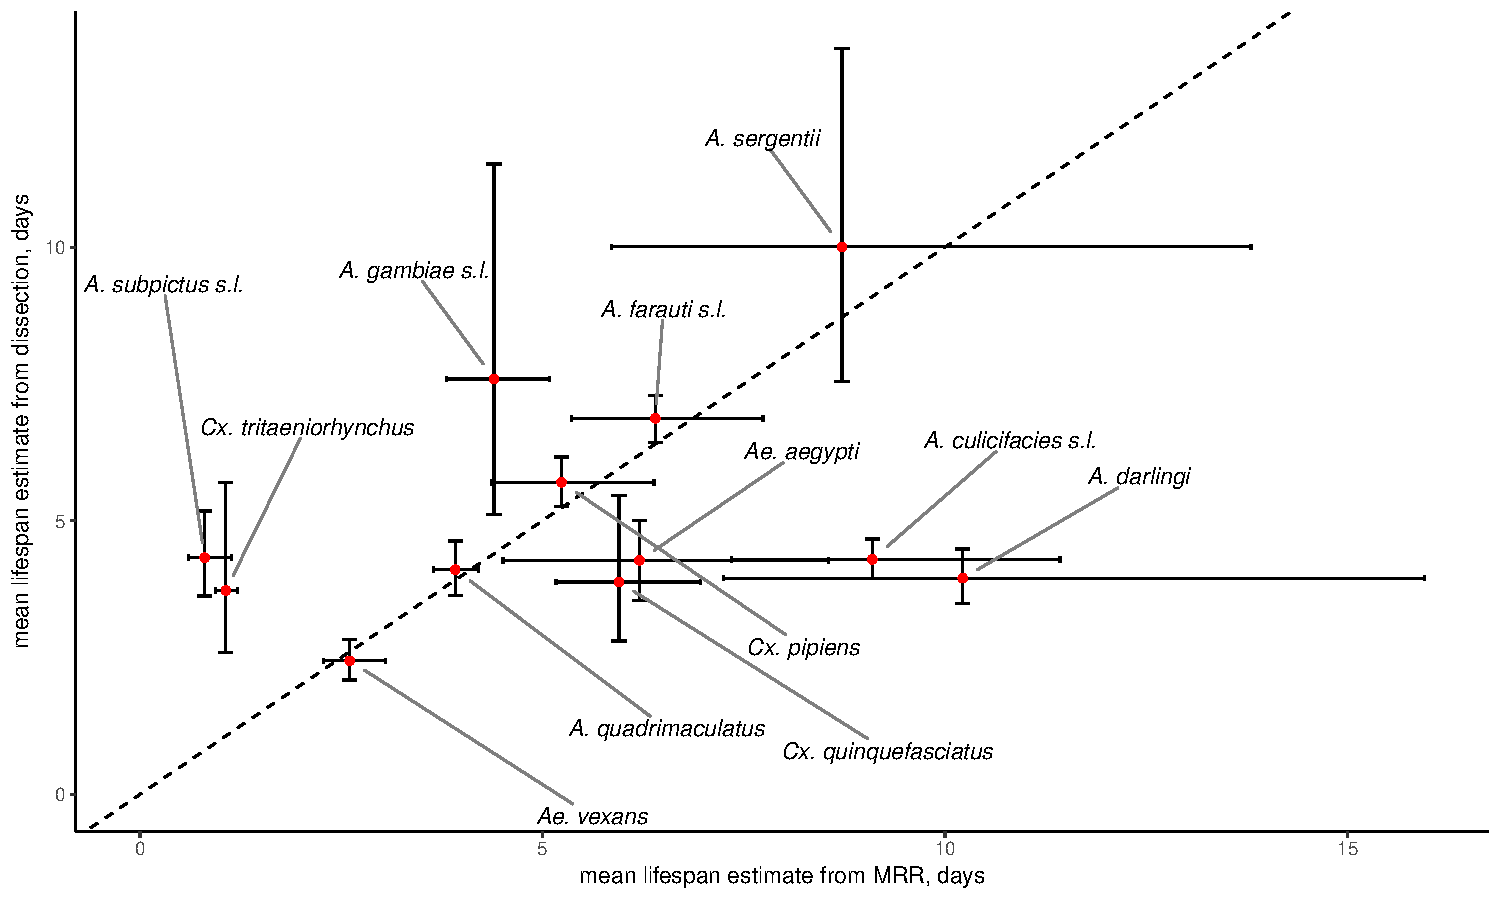
\includegraphics[width=1.3\textwidth]{./Figure_files/comparison.pdf}}
	\caption{\textbf{Comparison of estimates of female mosquito lifespan between MRR and dissection data.} For the MRR data, we show estimates for females that were neither fed with sugar or blood pre-release. The red points indicate the posterior mean estimates and the whiskers show the 25\% and 75\% quantiles. In both cases, the estimates were produced using the exponential survival model.}
	\label{fig:comparison}
\end{figure}

\begin{figure}[h]
	\centerline{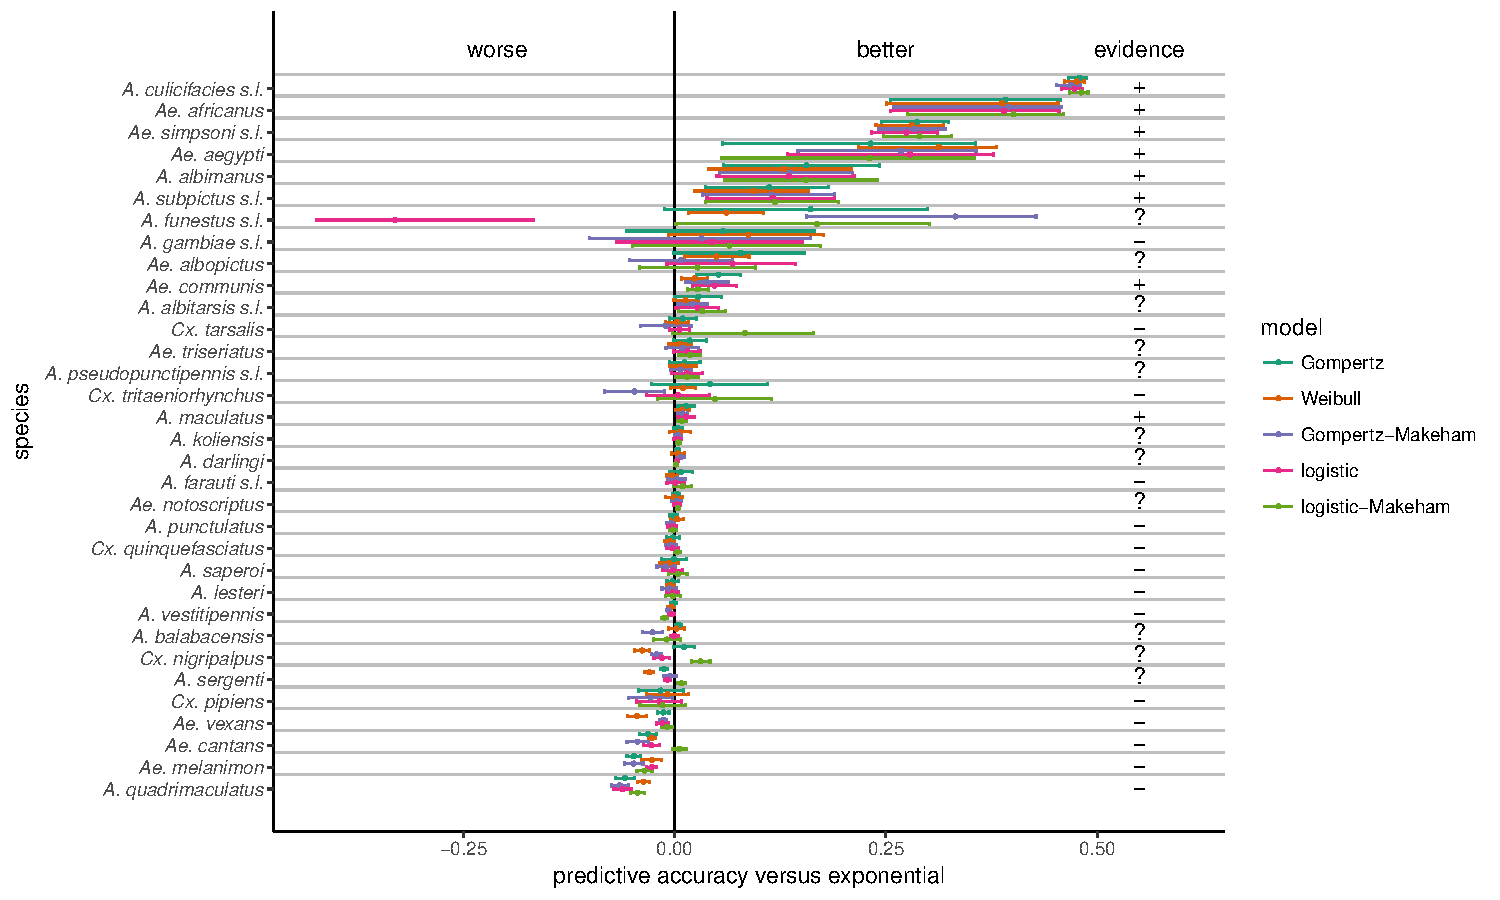
\includegraphics[width=1.3\textwidth]{./Figure_files/mrr_elpd_vs_exponential_ordered.pdf}}
	\caption{\textbf{Predictive accuracy of age-dependent models of mortality versus the exponential model by species for the MRR analysis.} The predictive accuracy was determined using K-Fold cross-validation as described in SOM; the measure of accuracy presented here by the central dots is the difference in estimated expected log pointwise predictive density compared to the exponential model. The lower and upper whiskers represent the lower and upper bounds of the 95\% confidence interval in predictive accuracy. The species have been ordered so that those with the highest average predictive accuracy across all age-dependent models compared to the exponential model appear at the top. If all age-dependent models outperform the exponential, we deem this as evidence for age-dependent mortality (`+'); if a subsample of models perform better, we deem the evidence ambiguous (`?'); and if no age-dependent model exceeds the performance of the exponential, we conclude no evidence in favour of senescence (`-').}
	\label{fig:mrr_elpd}
\end{figure}

\begin{figure}[h]
	\centerline{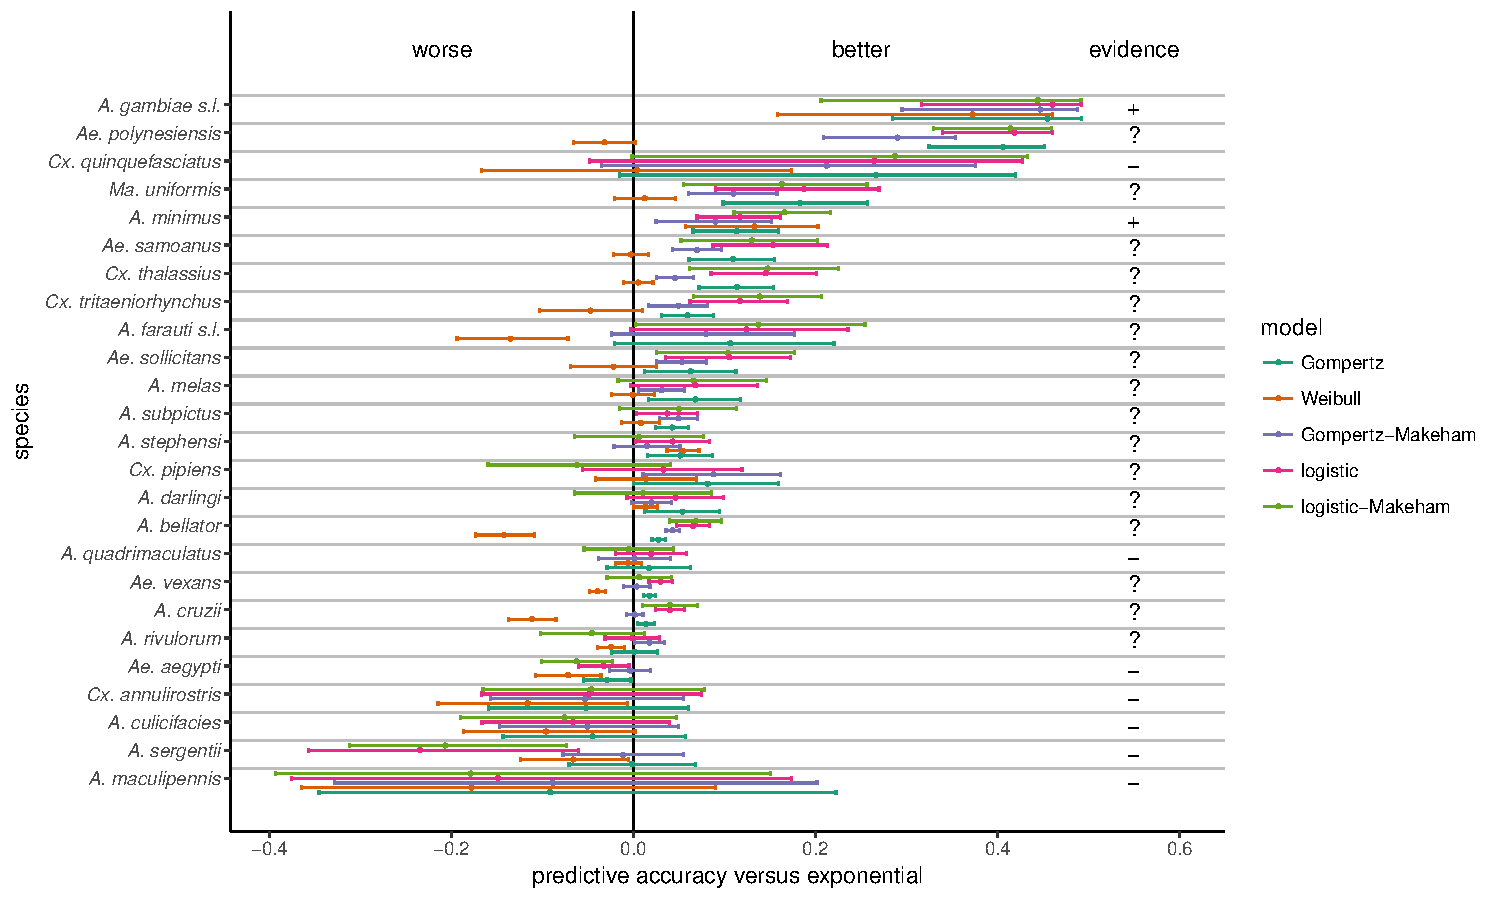
\includegraphics[width=1.3\textwidth]{./Figure_files/dissection_elpd_vs_exponential_ordered.pdf}}
	\caption{\textbf{Predictive accuracy of age-dependent models of mortality versus the exponential model by species for the dissection analysis.} The predictive accuracy was determined using K-Fold cross-validation as described in SOM; the measure of accuracy presented here by the central dots is the difference in estimated expected log pointwise predictive density compared to the exponential model. The lower and upper whiskers represent the lower and upper bounds of the 95\% confidence interval in predictive accuracy. The species have been ordered so that those with the highest average predictive accuracy across all age-dependent models compared to the exponential model appear at the top. If all age-dependent models outperform the exponential, we deem this as evidence for age-dependent mortality (`+'); if a subsample of models perform better, we deem the evidence ambiguous (`?'); and if no age-dependent model exceeds the performance of the exponential, we conclude no evidence in favour of senescence (`-').}
	\label{fig:dissection_elpd}
\end{figure}

\begin{figure}[h]
	\centerline{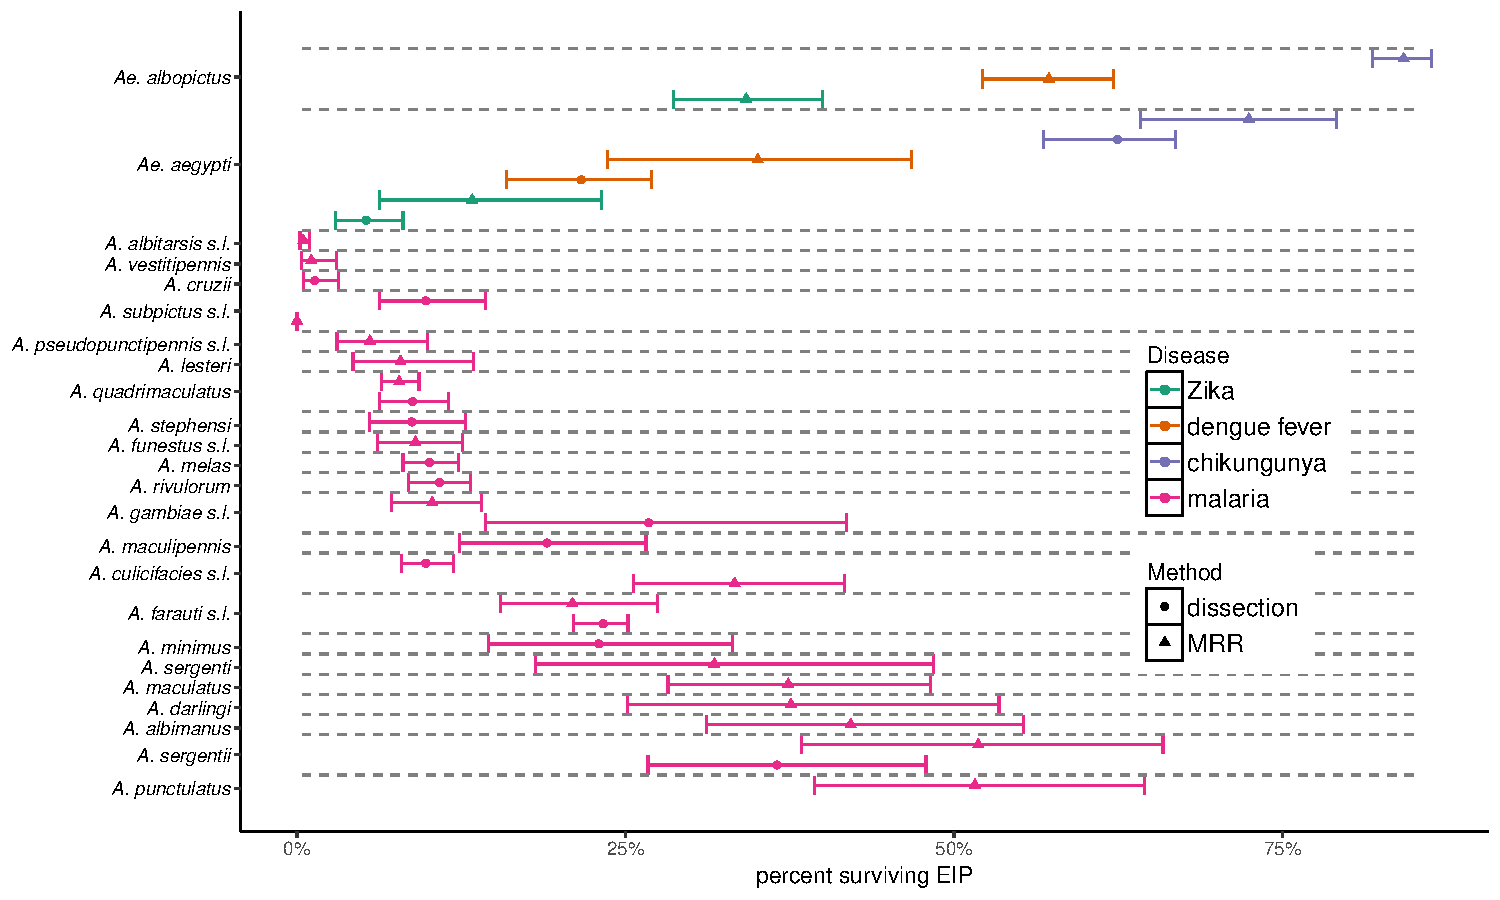
\includegraphics[width=1.3\textwidth]{./Figure_files/eip_all_combined.pdf}}
	\caption{\textbf{The MRR and dissection analyses estimates of the proportion of mosquitoes surviving the EIP of malaria, chikungunya, dengue fever and Zika for the disease vectors in our sample.} We assumed that the EIPs were: malaria-10 days, chikungunya-2 days, dengue fever-6.5 days and Zika-12.5 days. The left and right whiskers indicate the 25\% and 75\% posterior quantiles, and the points indicate the mean. All estimates were obtained using the exponential survival model.}
	\label{fig:eip}
\end{figure}


 \bibliographystyle{authordate1}
 \bibliography{Malaria}
\newpage

\end{document}